\documentclass[11pt,letterpaper]{article}
\usepackage[margin=0.85in,headheight=14pt]{geometry}
\usepackage{amsmath,amssymb}
\usepackage{enumitem}
\usepackage{fancyhdr}
\usepackage{lmodern}
\usepackage[T1]{fontenc}
\usepackage[dvipsnames]{xcolor}
\usepackage[most]{tcolorbox}
\usepackage{pgfplots}
\usepgfplotslibrary{groupplots}
\usetikzlibrary{arrows.meta,positioning,shapes.geometric}
\pgfplotsset{
  compat=1.18,
  every axis/.append style={grid=major, grid style={gray!25}, tick label style={font=\footnotesize},
    label style={font=\small}, title style={font=\small}, legend style={font=\scriptsize}},
}
\definecolor{cA}{HTML}{1F77B4}
\definecolor{cB}{HTML}{FF7F0E}
\definecolor{cC}{HTML}{2CA02C}
\definecolor{cD}{HTML}{D62728}
\definecolor{cE}{HTML}{9467BD}

\pagestyle{fancy}
\fancyhf{}
\lhead{SYDE 556/750 \qquad Test 1}
\rhead{Solutions \& marking guide}
\cfoot{\thepage}
\renewcommand{\headrulewidth}{0pt}

\setlength{\parindent}{0pt}
\setlength{\parskip}{4pt}

\newcommand{\tref}{\tau_{\mathrm{ref}}}
\newcommand{\trc}{\tau_{RC}}
\newcommand{\T}{\mathsf T}
\newcommand{\Jb}{J^{\mathrm{bias}}}
\newcommand{\ans}[1]{\par\vspace{4pt}{\bfseries #1}\quad}

\newtcolorbox{marking}{colback=blue!3,colframe=blue!40!black,boxrule=0.4pt,left=4pt,right=4pt,top=2pt,bottom=2pt,arc=1pt,fonttitle=\bfseries\small,title=Marking}
\newtcolorbox{trap}{colback=red!4,colframe=red!50!black,boxrule=0.4pt,left=4pt,right=4pt,top=2pt,bottom=2pt,arc=1pt,fonttitle=\bfseries\small,title=Where marks are usually lost}

\begin{document}

\begin{center}
{\Large\bfseries Test 1: Neurons \& Population Representation --- Solutions}\\[2pt]
Total: 20 marks plus 2 bonus. Simulation data: \texttt{tests\_data/make\_data.py}.\\
Mark splits are inferred from the marked paper where possible.
\end{center}

%=====================================================================
\section*{Question 1 \hfill (4)}
With $e = +1$, the current is $J = \alpha x + \Jb$ and the rate is $a = \max(J, 0)$. Two conditions fix the two unknowns.
\begin{itemize}[leftmargin=1.2em]
\item The neuron starts firing at $x = \xi$, so the current is zero there: $\alpha\xi + \Jb = 0$.
\item It fires at $a^{\max}$ at $x = 1$. Since $G$ is the identity for $J > 0$, $G^{-1}[a^{\max}] = a^{\max}$, so $\alpha + \Jb = a^{\max}$.
\end{itemize}
Subtracting the first equation from the second gives $\alpha(1 - \xi) = a^{\max}$:
\[
\boxed{\ \alpha = \frac{a^{\max}}{1 - \xi}, \qquad \Jb = -\alpha\xi = -\frac{\xi\,a^{\max}}{1 - \xi}\ }
\qquad\Longrightarrow\qquad a(x) = a^{\max}\,\frac{\max(x - \xi,\,0)}{1 - \xi}.
\]
Check: $a(\xi) = 0$ and $a(1) = a^{\max}$. For $e = -1$, replace $x$ by $ex$ and $\xi$ by $e\xi$.
\begin{center}
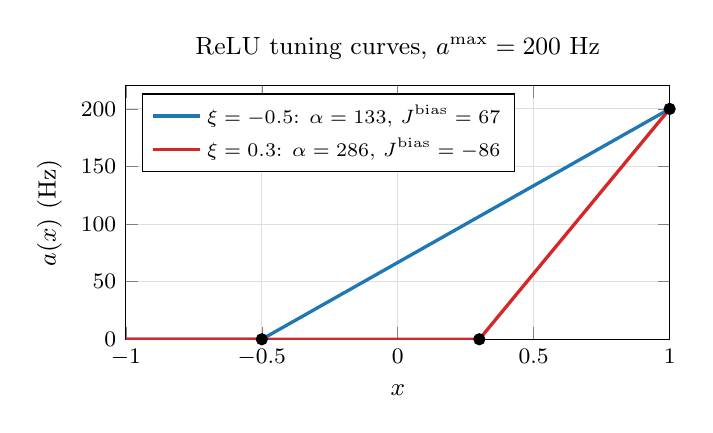
\begin{tikzpicture}
\begin{axis}[width=0.7\textwidth, height=4.8cm, xmin=-1, xmax=1, ymin=0, ymax=220,
  xlabel={$x$}, ylabel={$a(x)$ (Hz)}, legend pos=north west, legend cell align=left,
  title={ReLU tuning curves, $a^{\max} = 200$ Hz}]
  \addplot[cA, very thick, domain=-1:1, samples=201] {200*max(x+0.5,0)/1.5};
  \addplot[cD, very thick, domain=-1:1, samples=201] {200*max(x-0.3,0)/0.7};
  \legend{{$\xi = -0.5$: $\alpha = 133$, $\Jb = 67$}, {$\xi = 0.3$: $\alpha = 286$, $\Jb = -86$}}
  \addplot[only marks, mark=*, black] coordinates {(-0.5,0) (0.3,0) (1,200)};
\end{axis}
\end{tikzpicture}
\end{center}
\begin{marking}
1: intercept condition $\alpha\xi + \Jb = 0$. \ 1: maximum-rate condition $\alpha + \Jb = a^{\max}$ (noting $G^{-1}$ is the identity for ReLU). \ 1: $\alpha$. \ 1: $\Jb$.
\end{marking}
\begin{trap}
Copying the LIF recipe, where the threshold current is $1$ rather than $0$. For LIF the conditions are $\alpha\xi + \Jb = 1$ and $\alpha + \Jb = G^{-1}[a^{\max}]$.
\end{trap}

%=====================================================================
\section*{Question 2 \hfill (4)}
LIF tuning curves are not straight lines. Each one is zero up to its intercept, then rises with a near-vertical slope, then bends over (concave) as the rate approaches the $1/\tref$ ceiling. All three reach the same $a^{\max}$ at the end of the range in their preferred direction: $x = +1$ for $e = +1$, and $x = -1$ for $e = -1$.
\begin{center}
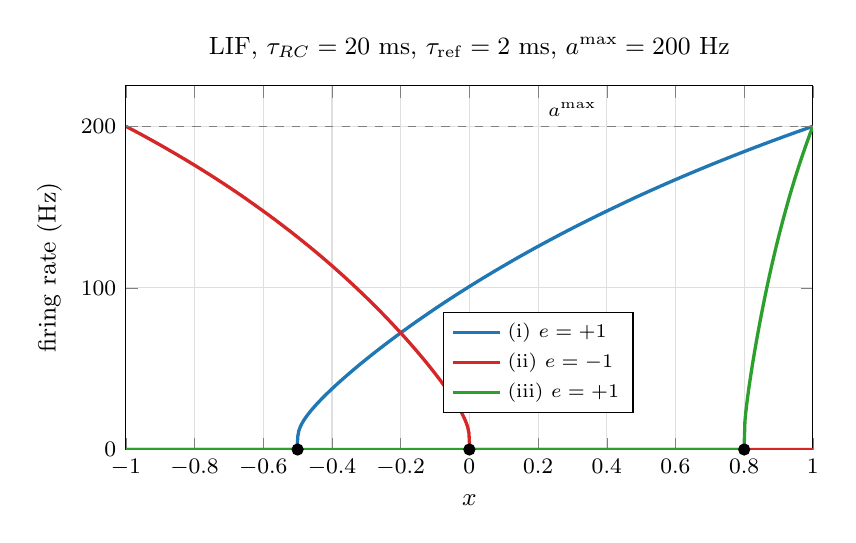
\begin{tikzpicture}[
  declare function={lif(\z,\tr,\tc,\Jm) = (\z > 0) * 1/(\tr - \tc*ln(1 - 1/(1 + (\Jm-1)*max(\z,1e-6))));}]
\begin{axis}[width=0.85\textwidth, height=6.2cm, xmin=-1, xmax=1, ymin=0, ymax=225,
  xlabel={$x$}, ylabel={firing rate (Hz)}, legend style={at={(0.6,0.1)}, anchor=south}, legend cell align=left,
  title={LIF, $\trc = 20$ ms, $\tref = 2$ ms, $a^{\max} = 200$ Hz}]
  \addplot[cA, very thick, domain=-1:1, samples=800] {lif((x+0.5)/1.5,0.002,0.02,7.1792)};
  \addplot[cD, very thick, domain=-1:1, samples=800] {lif(-x,0.002,0.02,7.1792)};
  \addplot[cC, very thick, domain=-1:1, samples=800] {lif((x-0.8)/0.2,0.002,0.02,7.1792)};
  \legend{(i) $e = +1$, (ii) $e = -1$, (iii) $e = +1$}
  \addplot[only marks, mark=*, black, forget plot] coordinates {(-0.5,0) (0,0) (0.8,0)};
  \node[font=\scriptsize, anchor=north] at (axis cs:-0.5,-3) {$-0.5$};
  \node[font=\scriptsize, anchor=north] at (axis cs:0,-3) {$0$};
  \node[font=\scriptsize, anchor=north] at (axis cs:0.8,-3) {$0.8$};
  \draw[dashed, gray] (axis cs:-1,200) -- (axis cs:1,200);
  \node[font=\scriptsize, anchor=south] at (axis cs:0.3,200) {$a^{\max}$};
\end{axis}
\end{tikzpicture}
\end{center}
Curve (iii) has only $0.2$ of input range to climb from $0$ to $a^{\max}$, so it is by far the steepest. Curve (ii) is the mirror image of an $e = +1$ neuron with intercept $0$.
\begin{marking}
1 per curve (3): correct direction (increasing for $e = +1$, decreasing for $e = -1$), zero on the non-firing side, intercept in the right place and labelled. \ 1: LIF shape, meaning a steep onset that flattens toward $a^{\max}$ and the same $a^{\max}$ for all three. Straight ReLU-style lines lose this mark.
\end{marking}
\begin{trap}
Drawing straight lines (ReLU shape), or drawing the LIF curve convex (flat at first, then steepening). The steepest part of an LIF curve is right at the intercept.
\end{trap}

%=====================================================================
\section*{Question 3 \hfill (4)}

\ans{(a) [1]}
Let $\mathbf A$ be $N \times M$ (row $i$ holds neuron $i$'s rates at the $M$ sample points) and $\mathbf x$ be the $1 \times M$ row of sample values. Then
\[
\boxed{\ \bigl(\mathbf A\mathbf A^\T + M\sigma^2\mathbf I\bigr)\,\mathbf d = \mathbf A\mathbf x^\T\ }
\qquad\text{i.e.}\qquad \mathbf d = \bigl(\mathbf A\mathbf A^\T + M\sigma^2\mathbf I\bigr)^{-1}\mathbf A\mathbf x^\T,
\]
with $\mathbf I$ the $N \times N$ identity. The noise term is multiplied by the number of \emph{samples}, because $\mathbf A\mathbf A^\T$ is a sum over the $M$ samples. The lecture notes write the same equation as $\mathbf D^\T = (\mathbf A\mathbf A^\T + N\sigma^2\mathbf I)^{-1}\mathbf A\mathbf X^\T$, but there $N$ is the number of samples and $n$ is the number of neurons.
\begin{marking}
0.5: least-squares form $\mathbf A\mathbf A^\T \mathbf d = \mathbf A\mathbf x^\T$. \ 0.5: the $\sigma^2\mathbf I$ term on the diagonal.
\end{marking}

\ans{(b) [2]}
\[
\hat{\mathbf x} = \mathbf D\,\mathbf a = \sum_{i=1}^{10} a_i\,\mathbf d_i,
\]
where column $i$ of $\mathbf D$ is neuron $i$'s 2-D decoding vector $\mathbf d_i$.
\begin{center}
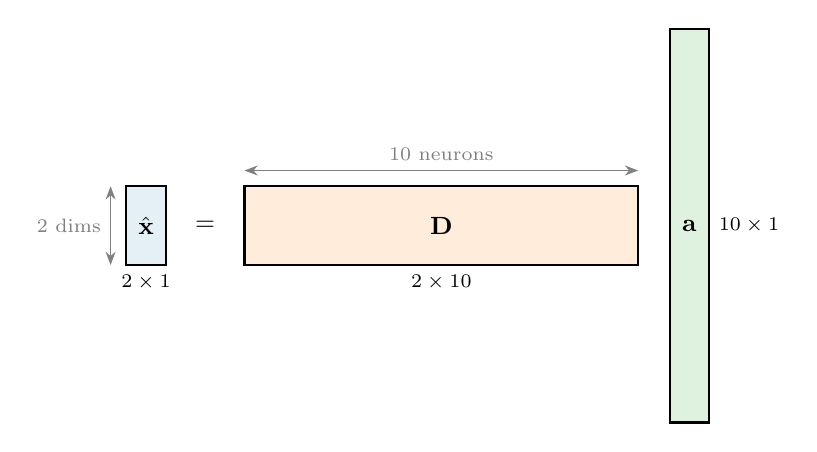
\begin{tikzpicture}[font=\small, u/.style={draw, thick, fill=cA!12}]
  \draw[u] (0,0) rectangle (0.5,1.0); \node at (0.25,0.5) {$\hat{\mathbf x}$};
  \node[below, font=\scriptsize] at (0.25,0) {$2 \times 1$};
  \node at (1.0,0.5) {$=$};
  \draw[u, fill=cB!15] (1.5,0) rectangle (6.5,1.0); \node at (4,0.5) {$\mathbf D$};
  \node[below, font=\scriptsize] at (4,0) {$2 \times 10$};
  \draw[u, fill=cC!15] (6.9,-2.0) rectangle (7.4,3.0); \node at (7.15,0.5) {$\mathbf a$};
  \node[right, font=\scriptsize] at (7.4,0.5) {$10 \times 1$};
  \draw[{Stealth}-{Stealth}, gray] (1.5,1.2) -- node[above, font=\scriptsize] {10 neurons} (6.5,1.2);
  \draw[{Stealth}-{Stealth}, gray] (-0.2,0) -- node[left, font=\scriptsize] {2 dims} (-0.2,1.0);
\end{tikzpicture}
\end{center}
If you solved for $\mathbf D^\T$ ($10 \times 2$) with the formula in (a), the decode is $\hat{\mathbf x} = (\mathbf D^\T)^\T\mathbf a$. The inner dimensions must match (10 with 10), and the result must be $2 \times 1$.
\begin{marking}
1: correct equation. \ 1: rectangles with correct, consistent dimensions ($2 \times 1 = (2 \times 10)(10 \times 1)$). Writing $\mathbf D$ as $10 \times 2$ in front of a $10 \times 1$ vector loses half a mark.
\end{marking}

\ans{(c) [1]}
Without the noise term, least squares fits the clean tuning curves almost exactly, using large decoders of alternating sign that cancel each other. When the activities are noisy, those large weights amplify the noise, since the noise error is $\sigma^2\|\mathbf d\|^2$. The $\sigma^2$ term penalizes large decoders (regularization). The result is smaller, more evenly spread decoders that average the noise out. They fit the clean curves slightly worse but give a much lower error on noisy activity.
\begin{center}
\begin{tikzpicture}
\begin{axis}[width=0.8\textwidth, height=5.4cm, xmin=-1, xmax=1, ymin=-1.3, ymax=1.3,
  xlabel={$x$}, ylabel={$\hat x$ from noisy $\mathbf a$}, legend pos=north west, legend cell align=left,
  title={20 LIF neurons, noise $\sigma = 0.1 \times 200$ Hz}]
  \addplot[cD, thin] table[x=x, y=plain] {tests_data/t1q3_noise.dat};
  \addplot[cA, thick] table[x=x, y=reg] {tests_data/t1q3_noise.dat};
  \addplot[black, dashed, domain=-1:1, samples=2] {x};
  \legend{without noise term (RMSE $0.117$), with noise term (RMSE $0.064$), ideal}
\end{axis}
\end{tikzpicture}
\end{center}
On clean activity the order flips: RMSE is $0.008$ without the noise term and $0.021$ with it. Regularization trades a little distortion for much better robustness to noise.
\begin{marking}
0.5: the term penalizes or shrinks the decoders (regularization). \ 0.5: smaller decoders amplify noise less, so the decode is more robust and has lower error when activities are noisy.
\end{marking}

%=====================================================================
\section*{Question 4 \hfill (4)}

\ans{(a) [1]}
Error due to \textbf{static distortion} ($E_{\mathrm{dist}}$) and error due to \textbf{noise} ($E_{\mathrm{noise}}$):
\[
E = \underbrace{\tfrac12\int_{-1}^{1}\bigl(x - \textstyle\sum_i d_i a_i(x)\bigr)^2 dx}_{E_{\mathrm{dist}}} + \underbrace{\tfrac12\sigma^2\textstyle\sum_i d_i^2}_{E_{\mathrm{noise}}}.
\]

\ans{(b) [2]}
In squared error, $E_{\mathrm{noise}} \propto 1/n$ and $E_{\mathrm{dist}} \propto 1/n^2$. (In RMSE these become $1/\sqrt n$ and $1/n$.)
\begin{center}
\begin{tikzpicture}
\begin{loglogaxis}[width=0.8\textwidth, height=6cm, xmin=3, xmax=1300,
  xlabel={number of neurons $n$}, ylabel={squared error}, legend pos=south west, legend cell align=left,
  title={LIF population, rates $100$--$200$ Hz, $\sigma = 20$ Hz (10 seeds per point)}]
  \addplot[cA, very thick, mark=*] table[x=n, y=noise] {tests_data/t1q4_errors.dat};
  \addplot[cD, very thick, mark=square*] table[x=n, y=dist] {tests_data/t1q4_errors.dat};
  \addplot[cA, dashed, domain=3:1300, samples=2] {0.072/x};
  \addplot[cD, dashed, domain=3:1300, samples=2] {0.46/x^2};
  \legend{$E_{\mathrm{noise}}$, $E_{\mathrm{dist}}$, $\propto 1/n$, $\propto 1/n^2$}
\end{loglogaxis}
\end{tikzpicture}
\end{center}
For any reasonably sized population, noise is the dominant source of error.

\ans{(c) [1]}
Noise is independent across neurons, so the decoder averages $n$ independent noise sources and the variance falls only as $1/n$. Distortion is a systematic fitting error: more neurons give more basis functions, so the curved tuning curves combine into a closer fit of $x$, and that residual shrinks faster, as $1/n^2$.
\begin{marking}
(a) 0.5 per source. \ (b) 1 per correct scaling. \ (c) 1: noise is averaged as independent random error, while distortion is reduced by a better fit from more basis functions.
\end{marking}

%=====================================================================
\section*{Question 5 \hfill (4)}
\textit{Page 3 of the paper (Question~5 and the bonus question) was not photographed. Add the question text to \texttt{556\_Test1\_neurons\_population.tex} and its solution here.}

\section*{Bonus Question 1 \hfill (2)}
\textit{See above.}

\end{document}
